% !TEX root = ./Vorlesungsmitschrift AGLA 2.tex  
\lecture{Di 02.06. 10:15}{}
Eine Rechtfertigung der Definition des Begriffs \enquote{projektive Basis}:
\begin{satz}\label{projektive_basen_sind_basig}
  Seien \( V,W \) \( K \)-Vektorräume mit \( \projectivedim{V}=\projectivedim{W}=n \) und \( (p_0,\dotsc,p_{n+1}) \) \bzw \( q_0,\dotsc,q_{n+1}  \) projektive Basen von \( \projectionspace{V} \) \bzw \( \projectionspace{W} \).

  Dann gibt es genau eine Projektivität
  \begin{equation*}
    f\maps \projectionspace{V}\to \projectionspace{W}
  \end{equation*}
  mit \( f(p_i)=q_i \), \( 0\leq i\leq n+1 \).
\end{satz}
\begin{bemerkung*}
  Ist \( \projectivedim{V}= \projectivedim{W}\), dann ist jede projektive Abbildung \( f\maps \projectionspace{V}\to \projectionspace{W}  \) eine Projektivität.
\end{bemerkung*}
\begin{proof}[Beweis von \thref{projektive_basen_sind_basig}]
  Wähle nach \thref{kanonische_projektive_basis_klappt} Basen \( v_0,\dotsc,v_n \) von \( V \) und \( w_0,\dotsc,w_n \) von \( W \) mit
  \begin{gather*}
    p_i=Kv_i\quad 0\leq i\leq n\\
    p_{n+1}=K(v_0+\dotsb+v_n)
  \end{gather*}
  und
  \begin{gather*}
    q_i=Kw_i\quad 0\leq i\leq n\\
    q_{n+1}=K(w_0+\dotsb+w_n).
  \end{gather*}
  Sei \( f\maps \projectionspace{V}\to\projectionspace{W} \) eine projektive Abbildung mit \( f(p_i)=q_i \), \( 0\leq i\leq n+1 \) und \( F\maps V\to W  \) eine zugehörige lineare Abbildung. Aus \( f(p_i)=q_i \) folgt für \( 0\leq i\leq n \)
  \begin{equation*}
    f(p_i)=K\cdot F(v_i)=q_i=K\cdot w_i,
  \end{equation*}
  also \texists \( \lambda_0,\dotsc,\lambda_n\in \fieldwithoutzero{K} \) mit
  \begin{equation*}
    F(v_i)=\lambda_i w_i\logicspace 0\leq i\leq n.
  \end{equation*}
  Aus 
  \begin{equation*}
    K\cdot F(v_0+\dotsb+v_n)=f(p_{n+1})=q_{n+1}=K\cdot (w_0+\dotsb+w_{n})
  \end{equation*}
  erhalten wir \( \lambda_{n+1}\in \fieldwithoutzero{K} \) mit
  \begin{equation*}
    \lambda_0 w_0+\dotsb+\lambda_n w_n = F(v_0+\dotsb+v_n)=\lambda_{n+1}(w_0+\dotsb+w_n).
  \end{equation*}
  Die Vektoren \( w_0,\dotsb,w_n\in W \) sind linear unabhängig, also ist
  \begin{equation*}
    \lambda_{n+1}=\lambda_0=\dotsb=\lambda_n.
  \end{equation*}
  Damit ist \( F\maps V\to W  \) als lineare Abbildung bis auf Skalieren mit \( \lambda_{n+1}\in \fieldwithoutzero{K} \) eindeutig bestimmt und damit \( f=\projectionmap{F} \) eindeutig bestimmt. Umgekehrt ist die Abbildung \( F\maps W\to V \) gegeben durch \( v_i\mapsto w_i \), \( 0\leq i\leq n \) ein Isomorphismus und \( \projectionmap{F}\maps \projectionspace{V}\to \projectionspace{W} \) hat die Eigenschaft, dass
  \begin{equation*}
    \projectionmap{F}(p_i)=q_i\quad 0\leq i\leq n+1.
  \end{equation*}
\end{proof}
\file{Projektivitäten beschrieben durch Matrizen}
\begin{frage*}
  Können wir Projektivitäten durch Matrizen beschreiben (ähnlich wie wir es für affine Abbildungen zwischen affinen Räumen gesehen haben)?
\end{frage*}
\tto Wir benötigen die Wahl eines Koordinatensystems.

Sei \( V \) ein \( n+1 \)-dimensionaler \( K \)-Vektorraum mit Basis \( v_0,v_1,\dotsc,v_n \). Dann ist
\begin{gather*}
  q_i=Kv_i\quad 0\leq i\leq n\\
  q_{n+1}=K(v_0+\dotsb+v_n).
\end{gather*}
eine projektive Basis von \( \projectionspace{V} \). Nach \thref{projektive_basen_sind_basig} gibt es eine eindeutig bestimmte Projektivität
\begin{equation*}
  \varphi\maps \projectionspaceover{n}{K}\to\projectionspace{V}
\end{equation*}
mit
\begin{gather*}
  \phi(p_i)=q_i \quad 0\leq i\leq n+1,
\end{gather*}
wobei
\begin{align*}
  p_0&=(1:\dotsc:0)\\
  &\vdots\\
  p_n&=(0:\dotsc:1)\\
  p_{n+1}&=(1:\dotsc:1)
\end{align*}
die kanonische Basis der \( \projectionspaceover{n}{K} \) ist.

\begin{definition*}
  Sei \( V \) ein \( K \)-Vektorraum und \( n=\projectivedim-{\projectionspace{V}} \). Unter einem Koordinatensystem von \( \projectionspace{V} \) verstehen wir eine Projektivität
  \begin{equation*}
    f\maps \projectionspaceover{n}{K}\to\projectionspace{V}.
  \end{equation*}
  Ist \( f(x_0:\dots:x_n)=p\in \projectionspace{V} \), dann nennen wir \( (x_0:\dotsc:x_n) \) einen homogenen Koordinatenvektor von \( p \).
\end{definition*}
\subsection*{Beschreibung von Projektivitäten durch Matrizen}
\begin{idee*}
  Seien \( V,W \) \( K \)-Vektorräume mit \( \dim-{V}=n+1 \) und
  \begin{equation*}
    f\maps \projectionspace{V}\to \projectionspace{W}
  \end{equation*}
  eine Projektivität. Wähle Koordinatensysteme
  \begin{equation*}
    \begin{tikzcd}
        \projectionspaceover{n}{K}\arrow[red,r,"g"]\arrow[shift right,d,"\varphi"{name=phi,left}]\arrow[shift left,d,dotted,yellow,"\varphi"] &\projectionspaceover{n}{K}X\arrow[shift left,d,"\psi"{name=psi}]\\
        \projectionspace{V}\arrow[shift left, r,"f",dotted,yellow]\arrow[shift right, r,"f"{below}]&\projectionspace{Y}\arrow[shift left, u,"\inverse{\psi}",yellow,dotted]
        \arrow[to path={(psi) node[midway,scale=1] {\rotatebox{90}{\(\circlearrowright\)}} (phi)}]   
    \end{tikzcd}
\end{equation*}
Dann ist \( g=\inverse{\psi}\circ f\circ \varphi \) Projektivität.

\end{idee*}
\begin{ziel*}
  Beschreibe \( g \) mit Hilfe der Sprache von Matrizen.
\end{ziel*}
Sei
\begin{equation*}
  G\maps K^{n+1}\to K^{n+1}
\end{equation*}
ein Isomorphismus mit \( g=\projectionmap{G} \) (\( G  \) ist bis auf Multiplikation mit Skalaren \( \neq 0 \) eindeutig bestimmt).

Dann besteht eine Matrix \( A\in \invertiblematrices{n+1}{K} \) mit \( G(\underline{x})=\underline{x} \) für alle
\begin{equation*}
  \underline{x}=(x_0,x_1,\dotsc,x_n)\in K^{n+1}.
\end{equation*}
Sei \( A=\parens*{a_{ij}}_{0\leq i,j\leq n} \). Es gilt
\begin{equation*}
  g(x_0:\dotsc:x_n)=\parens*{(a_{00}x_0+\dotsb+a_{0n}x_n):(a_{10}x_0+\dotsb+a_{1n}x_n):\dotsc:(a_{n0}x_0+\dotsb+a_{nn}x_n)}.
\end{equation*}
\begin{frage*}
  Wie verhält sich \( g \) eingeschränkt auf \( \iota(K^n) \)? 
\end{frage*}
Wir haben die kanonische Einbettung als
\begin{equation*}
  \begin{split}
    \iota\maps K^n&\to \projectionspaceover{n}{K}\setminus H\\
    (x_1,\dotsc,x_n)&\mapsto (1:x_1:\dotsc:x_n),
  \end{split}
\end{equation*}
definiert, mit
\begin{equation*}
  H=\Set{(y_0:y_1:\dotsc:y_n)\in \projectionspaceover{n}{K}|y_0=0}.
\end{equation*}
Es gilt für \( (x_1,\dotsc,x_n)\in K^n \).
\begin{equation*}
  g(\iota(x_1,\dotsc,x_n))=\parens{\underrelate{\vertrelation{\isittrue{=}}}{0}{a_{00}+a_{01}x_1+\dotsb+a_{0n}x_n}:a_{10}+a_{11}x_1+\dotsb:\dotsc:a_{n0}+a_{n1}x_1+\dotsb+a_{nn}x_n},
\end{equation*}
also \( g(\iota(x_1,\dotsc,x_n))\in \iota(K^n) \) genau dann, wenn
\begin{equation}
  a_{00}+a_{01}x_1+\dotsb+a_{0n}x_n\neq 0
\end{equation}
und in dem Fall ist
\begin{equation*}
  g(\iota(x_1,\dotsc,x_n))=\parens*{\frac{a_{10}+a_{11}x_1+\dotsb+a_{1n}x_n}{a_{00}+a_{01}x_1+\dotsb+a_{0n}x_n},\dotsc,\frac{a_{n0}+a_{n1}x_1+\dotsb+a_{nn}x_n}{a_{00}+a_{01}x_1+\dotsb+a_{0n}x_n}}.
\end{equation*}
\begin{bemerkung*}
  \( g \) induziert eine Abbildung
  \begin{equation*}
    \evaluateat{g}{\iota(K^n)}\maps \iota(K^n)\to \iota(K^n)\subseteq \projectionspaceover{n}{K}
  \end{equation*}
  genau dann, wenn
  \begin{equation*}
    a_{01}=\dotsb=a_{0n}=0.
  \end{equation*}
\end{bemerkung*}
\file{Zentralprojektionen}
\subsection*{Zentralprojektionen in der projektiven Geometrie}
Sei \( V \) ein \( K \)-Vektorraum, \( W,W_1,W_2\subseteq V \) \( K \)-Untervektorräume mit 
\begin{equation*}
  V=W\oplus W_1=W\oplus W_2,
\end{equation*}
dann sind \( Z=\projectionspace{W} \), \( Z_1=\projectionspace{W_1}  \) und \( Z_2=\projectionspace{W_2} \) projektive Unterräume von \( \projectionspace{V} \) mit
\begin{enumerate}
  \item \( Z\cap Z_1=Z\cap Z_2=\emptyset \) und 
  \item \( Z\vee Z_1=Z\vee Z_2=\projectionspace{V} \).
\end{enumerate}
Wir definieren eine Abbildung
\begin{equation*}
  \begin{split}
    f\maps Z_1&\to Z_2\\
    p&\mapsto (Z\vee p)\cap Z_2
  \end{split}
\end{equation*}
und nennen \( f \) \emph{Zentralprojektion}.
\begin{behauptung*}
  Für \( p\in Z_1 \) gilt
  \begin{equation*}
    \anzahl{(Z\vee p)\cap Z_2}=1.
  \end{equation*}
\end{behauptung*}
Denn wir berechnen
\begin{equation*}
  \projectivedim{(Z\vee p)\cap Z_2}
\end{equation*}
durch 
\begin{align*}
  \projectivedim{(Z\vee p)\cap Z_2}&\explain{\text{Dimensionsformel}}{=}\projectivedim{Z\vee p}+\projectivedim-{Z_2}-\projectivedim{Z\vee p\vee Z_2}\\
  &=\projectivedim{Z\vee p}+\projectivedim-{Z_2}-\projectivedim-{\projectionspace{V}}\\
  &=\projectivedim-{Z}+1+\projectivedim-{Z_2}-\projectivedim-{\projectionspace{V}}\\
  &=1-1=0
\end{align*}
also schneiden \( Z\vee p \) und \( Z_2 \) sich in genau einem Punkt.
\begin{figure}[H]
  \centering
  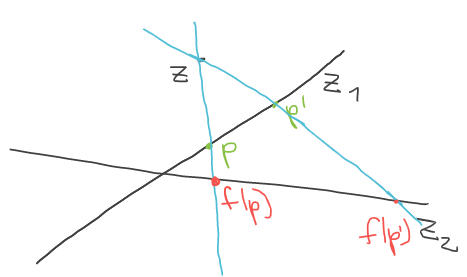
\includegraphics[width=0.5\linewidth]{zentralprojektion_einfaches_beispiel}
  \caption*{}
  \label{fig:zentralprojektion_einfaches_beispiel}
\end{figure}
\begin{lemma}
  Die oben definierte Zentralprojektion \( f \) ist eine Projektivität.
\end{lemma}
\begin{proof}
  Notation wie oben. Betrachte die Projektion von \( K \)-Vektorräumen
  \begin{equation*}
    \begin{split}
      P_W\maps V=W\oplus W_2&\to W_2\\
      w+w_2&\mapsto w_2.
    \end{split}
  \end{equation*}
  Dann ist
  \begin{equation*}
    \evaluateat{P_W}{W_1}\maps W_1\to W_2
  \end{equation*}
  ein Isomorphismus (siehe \ref{parallelprojektionen}). Also erhalten wir eine Projektivität
  \begin{equation*}
    \projectionmap{\evaluateat{P_W}{W_1}}\maps \equalto{Z_1}{\projectionspace{W_1}}\to \equalto{Z_2}{\projectionspace{W_2}}.
  \end{equation*}
  Sei \( p\in \projectionspace{W_1} \). Wir berechnen \( \projectionmap{\evaluateat{P_W}{W_1}}(p) \). Sei dazu \( p=K\cdot w_1 \) mit \( w_1\in W_1\setminus \zeroset \). Schreibe \( w_1=w+w_2 \) mit \( w\in W \), \( w_2\in W_2 \). Dann ist 
  \begin{equation*}
    \projectionmap{\evaluateat{P_W}{W_1}}(p)=K\cdot w_2\in Z_2.
  \end{equation*}
  Betrachte nun
  \begin{align*}
    (Z\vee p)\cap Z_2&=\projectionspace{W+K\cdot w_1}\cap \projectionspace{W_2}\\
    &=\projectionspace{W+K(w+w_2)}\cap \projectionspace{W_2}\\
    &=\projectionspace{W+K\cdot w_2}\cap \projectionspace{W_2}\\
    &=\projectionspace{(W+K\cdot w_2)\cap W_2}\\
    &\explain{W\cap W_2=\zeroset}{=}\projectionspace{K\cdot W_2}=K\cdot w_2.
  \end{align*}
  Also ist
  \begin{equation*}
    f(p)=K\cdot w_2=\projectionmap{\evaluateat{P_W}{W_1}}(p).
  \end{equation*}
  und damit
  \begin{equation*}
    f=\projectionmap{\evaluateat{P_W}{W_1}}
  \end{equation*}
  eine Projektivität.
\end{proof}